\chapter{Server}
Il passaggio principale che ho dovuto affrontare per l'inizio del progetto è stata l'inizializzazione
di un server che potesse gestire lo scambio di informazioni con l'applicazione ed occuparsi di svolgere tutti i compiti del caso.

Il lavoro del server è facilmente scomponibile in due parti, la gestione dei dati utili per la classificazione 
(che sarà poi affrontata nel capitolo \ref{chapter:classification}) e l'erogazione di dati informativi che vedremo consentire
ad un amministratore l'interazione con il sistema.

Si è scelto di sviluppare il tutto con il linguaggio Python e di inserire per comodità il software in due differenti contenitori Docker, in modo da 
mantenere differenziate queste due parti anche a livello programmativo.

\subsubsection{Docker}
Docker \cite{docker} è un progetto open-source in grado di effettuare il deploy di applicazioni all'interno di contenitori software che grazie alla
virtualizzazione si trovano ad un livello di astrazione differente dal sistema host. Questa tecnica è molto utile quando si vuole
mantenere separati l'installazione di un'applicativo dal sistema ospitante.



\section{RESTful Web API}
\label{section:api}
Come si intuisce in figura \ref{fig:overview}, si è pensato alla creazione di una RESTful Web API, ovvero un'interfaccia composta da un insieme
di \textit{endpoints} pubblici che consentono di ottenere delle informazioni.
Tutti i componenti interessati a tali informazioni sono in grado di ottenerle mediante un sistema di richiesta-risposta tra client e server. 

Si ha accesso ad informazioni sempre aggiornate. Un cambiamento dei valori in fase di amministrazione consente la 
distribuzione delle modifiche senza la necessità di rilasciare un aggiornamento dell'applicazione o riprogrammare il ricevitore.


\subsection{Protocollo e formato}
Tutte le richieste e le risposte utilizzano per lo scambio dati il protocollo HTTP, il comune protocollo di livello 
applicativo utilizzato nel World Wide Web.

I dati sono trasmessi con il formato JSON, uno standard che sfrutta una notazione chiave-valore facilmente leggibile.


\subsection{Endpoints}
Gli endpoints sono i punti in cui un software esterno accede a determinate informazioni. L'accesso avviene mediante la chiamata ad uno 
specifico URL che ci si aspetta risponda con i dati richiesti.

Gli endpoints che ho previsto sono riservati ad ottenere informazioni su
\begin{itemize}
    \item la lista delle attività classificabili
    \item la lista delle posizioni previste
    \item un modello per la richiesta di informazioni aggiuntive
\end{itemize}

\begin{listing}[H] 
    \begin{minted}[frame=single,framesep=10pt]{text}
http://IP_ADDRESS:PORT/activities
http://IP_ADDRESS:PORT/positions
http://IP_ADDRESS:PORT/form
    \end{minted}
    \caption{Elenco degli endpoints disponibili}
    \label{listing:endpoint-positions}
\end{listing}

\subsubsection{Lista delle attività}
Il primo degli endpoints impostato riguarda la lista di tutte le attività che il sistema imparerà a riconoscere.

Come è mostrato nel ritaglio di codice \ref{listing:response-activities}, la risposta di una chiamata a questo endpoint fornisce una lista 
di tutte le attività classificabili, ognuna contenente 
\begin{itemize}
    \item l'identificativo numerico
    \item il nome
    \item le traduzioni nelle lingue ammesse
    \item il tempo (in secondi) indicante la durata necessaria per l'addestramento
\end{itemize}

\newpage
\begin{listing}[H] 
    \inputminted[frame=single,framesep=10pt]{json}{assets/snippets/server/api/activities.json}
    \caption{Esempio di risposta dell'endpoint delle attività}
    \label{listing:response-activities}
\end{listing}

\newpage
\subsubsection{Lista delle posizioni del dispositivo}
Il secondo endpoint fornisce la lista di tutte le posizioni in cui può essere posizionato il dispositivo durante l'esecuzione 
di una analisi o di un apprendimento.

\begin{listing}[H] 
    \inputminted[frame=single,framesep=10pt]{json}{assets/snippets/server/api/positions.json}
    \caption{Esempio di risposta dell'endpoint delle posizioni}
\end{listing}

\newpage
\subsubsection{Modello per la richiesta di informazioni aggiuntive}
Il terzo endpoint fornisce una struttura per la generazione sull'applicazione di un modulo per la richiesta di dati aggiuntivi. 
Ne discuteremo meglio nel capitolo \ref{chapter:app}.

\begin{listing}[H] 
    \inputminted[frame=single,framesep=10pt]{json}{assets/snippets/server/api/form.json}
    \caption{Esempio di risposta dell'endpoint sui dati aggiuntivi}
\end{listing}

\subsection{Implementazione}
L'implementazione del software è stata effettuata con l'utilizzo di Flask. Si occupa di esporre i 
file JSON contenenti le informazioni appena viste nei rispettivi endpoints.

\subsubsection{Flask}
Flask \cite{flask} è uno dei più famosi framework per lo sviluppo di applicazioni web 
con Python. La sue caratteristiche principali sono leggerezza e semplicità, pur permettendo anche implementazioni 
più avanzate.


\begin{listing}[H] 
    \inputminted[frame=single,framesep=10pt]{python}{assets/snippets/server/api/flask.py}
    \caption{Flask App per una RESTful Web API con 3 endpoints}
\end{listing}



\section{Ricevitore}
\label{section:receiver}
Sempre da figura \ref{fig:overview} è possibile intuire che sul server trovano luogo anche il classificatore, 
i dati che sono stati raccolti e tutti i modelli generati. 

In questa sezione ci occuperemo di ciò che riguarda l'applicativo riservato a gestire la ricezione dei dati e fornire le risposte. 
In particolare la parte del software che si occupa di accettare le connessioni dai client (idealmente l'applicazione realizzata, di cui 
discuteremo nel capitolo \ref{chapter:app}) e di immagazzinare i dati ottenuti.

\subsection{Protocollo e formato}
Avendo la necessità di trasmettere i dati con il minimo ritardo, la connessione al ricevitore avviene via socket mediante TCP.
Essendo un protocollo di rete a livello di trasporto ci consente di avere una velocità maggiore rispetto a HTTP. 

Per comodità si continua ad utilizzare il formato JSON anche in questo frangente per organizzare le informazioni durante lo scambio dati.


\subsection{Messaggi}
Il ricevitore deve gestire due tipi di richieste, quelle che inviano i dati per effettuarne l'apprendimento e quelle che inviano
i dati in attesa di ricevere il risultato di una classificazione. Malgrado ciò la lettura dei messaggi ricevuti resta la medesima ed il 
valore per identificare la tipologia di richiesta è disponibile internamente alle informazioni.
\vspace{5mm} %5mm vertical space
\newline
Come mostrato nell'esempio \ref{listing:example-message-learning}, oltre alle informazioni sul tipo di richiesta, un singolo messaggio contiene 
\begin{itemize}
    \item un codice identificante un gruppo di messaggi
    \item un indice indicante la progressione dei dati
    \item i valori dei 3 assi (x, y, z)
    \item il sensore di movimento che ha generato i valori ottenuti
    \item un valore temporale (\textit{timestamp})
    \item la posizione del telefono selezionata durante l'attività in corso
\end{itemize}
e, in aggiunta, nel caso dell'apprendimento\dots
\begin{itemize}
    \item l'attività che si sta svolgendo
\end{itemize}

\begin{listing}[H] 
    \inputminted[frame=single,framesep=10pt]{json}{assets/snippets/server/receiver/message.json}
    \caption{Esempio di messaggio ricevuto per l'apprendimento}
    \label{listing:example-message-learning}
\end{listing}

\newpage
\subsection{Azioni}
Le azioni da intraprendere per le diverse tipologie di richiesta sono differenti. 

\subsubsection{Messaggi di Apprendimento}
Nel caso della ricezione di dati per l'apprendimento è necessario procedere al salvataggio degli stessi.

\vspace{5mm} %5mm vertical space
I record vengono suddivisi sulla base del relativo sensore. Per ogni sensore si genera un file CSV contenente i record con tutte 
le informazioni rimanenti.

\begin{figure}[H]
    \centering
    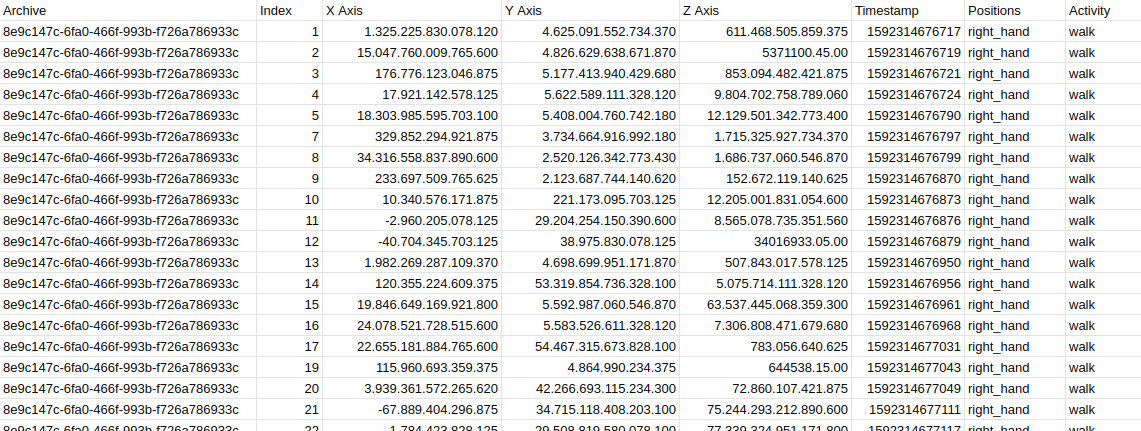
\includegraphics[scale = 0.39]{assets/images/examples/dataset-data-example.png}
    \caption{Esempio del dataset CSV contenente dati accelerometrici}
    \label{fig:example-dataset-csv-accelerometer}
\end{figure}

Ogni volta che la base di dati subisce delle modifiche si avvia il processo di \textit{train} del classificatore, 
trattato nel capitolo \ref{chapter:classification}.


\subsubsection{Messaggi di Analisi}
Nel caso di ricezione di dati per l'analisi non si deve immagazzinare le informazioni ricevute. 
L'obiettivo di questa fase è quello di fornire in risposta al client l'informazione che si aspetta.

Alla ricezione di un numero minimo di record si avvia il processo di classificazione, trattato sempre nel capitolo \ref{chapter:classification}.
L'ipotesi ottenuta dal classificatore sarà inviata come risposta.

\begin{listing}[H] 
    \inputminted[frame=single,framesep=10pt]{json}{assets/snippets/server/receiver/prediction.json}
    \caption{Esempio del messaggio di risposta con l'ipotesi formulata}
\end{listing}